\chapter{Algorithmic Aspects of k-Trees}

\begin{quotation}
In this chapter, we review basic definitions and properties of a hierarchy of graph classes known as $k$-trees, where $k\geq 1$. Several important classes of graphs are known to be special cases of partial $k$-trees, for $k=1,2,3$, and $4$. Also, several NP-complete problems have been shown to admit polynomial time algorithms on partial $k$-trees, when $k$ is fixed. Our main contributions in the next chapters show that the probabilistic connectivity problems introduced in Chapter 1 also admit similar polynomial time algorithms. As an introduction to the algorithmic ideas used in subsequent chapters, we review an algorithm due to \cite{wald1983steiner} for solving the Steiner tree problem on partial 2-trees. We conclude by discussing known results on extracting a partial $k$-tree subgraph, with prescribed $k$, from an arbitrary given network.
\end{quotation}

\section{Graph Notation}
\label{sec:graphNotation}

In this section, we introduce a few graph theoretic notations that we need throughout the thesis. In general, we adopt the same notation used, for example, in \cite{cormen2001introduction} and other books. 
An undirected graph $G=(V,E)$ has a set $V$ of \textit{nodes} (or vertices), and a set $E$ of \textit{edges} (or links).
We also use $V(G)$ and $V_G$ to denote the set of nodes. Likewise, we use $E(G)$ and $E_G$ to denote the set of edges. \\
We also need the following notation.
\begin{itemize}[noitemsep]
\item $deg_G(v)$: the degree of node $v$ in graph $G$
\item $N_G(v)$: the set of neighbouring nodes of $v$ in $G$
\item An \textit{induced subgraph} $G'\subseteq G$ on a set $V'\subseteq V$ of nodes contains all edges of $G$ where the two end nodes of each edge lie in $V'$.
\item A clique is a complete graph, and a $k$-clique is a clique on $k$ nodes.
\item A separator in $G$ is a subset of nodes whose removal disconnects $G$ into two, or more, connected components.
\end{itemize}


\section{$k$-Trees and Partial $k$-Trees}
\label{sec:ktree}
{\bf $k$-Trees.} The formulation of $k$-trees dates back to the work of \cite{beineke1969number, beineke1968enumeration} as a generalization of conventional trees. A recursive definition is given below.
\begin{definition} For a given integer $k\geq 1$, the class of $k$-trees is defined as follows
\begin{enumerate}[noitemsep]
\item A $k$-clique is a $k$-tree.
\item If $G_n$ is a $k$-tree on $n$ nodes then so is the graph $G_{n+1}$ obtained by adding a new node, and making it adjacent to every node in $k$-clique of $G_n$. $\blacksquare$
\end{enumerate}
\end{definition}

Thus, trees are 1-trees. A \textit{$k$-leaf} of a $k$-tree $G$ on $k+1$, or more, nodes is a node whose neighbours induce a $k$-clique. By repeatedly deleting $k$-leaves form a $k$-tree $G_n$, on $n\ge k$ nodes, one can reduce $G_n$ to a $k$-clique. We call such a sequence of nodes a \textit{$k$-leaf elimination sequence}.
\begin{example}
\normalfont
Figure \ref{fig:f3t1} illustrates a fragment of $3$-tree $G$ on $n=6$ nodes. $G$ has a $3$-leave $v_b$. $\blacksquare$
\end{example}
\begin{figure}[!htb]
\centering
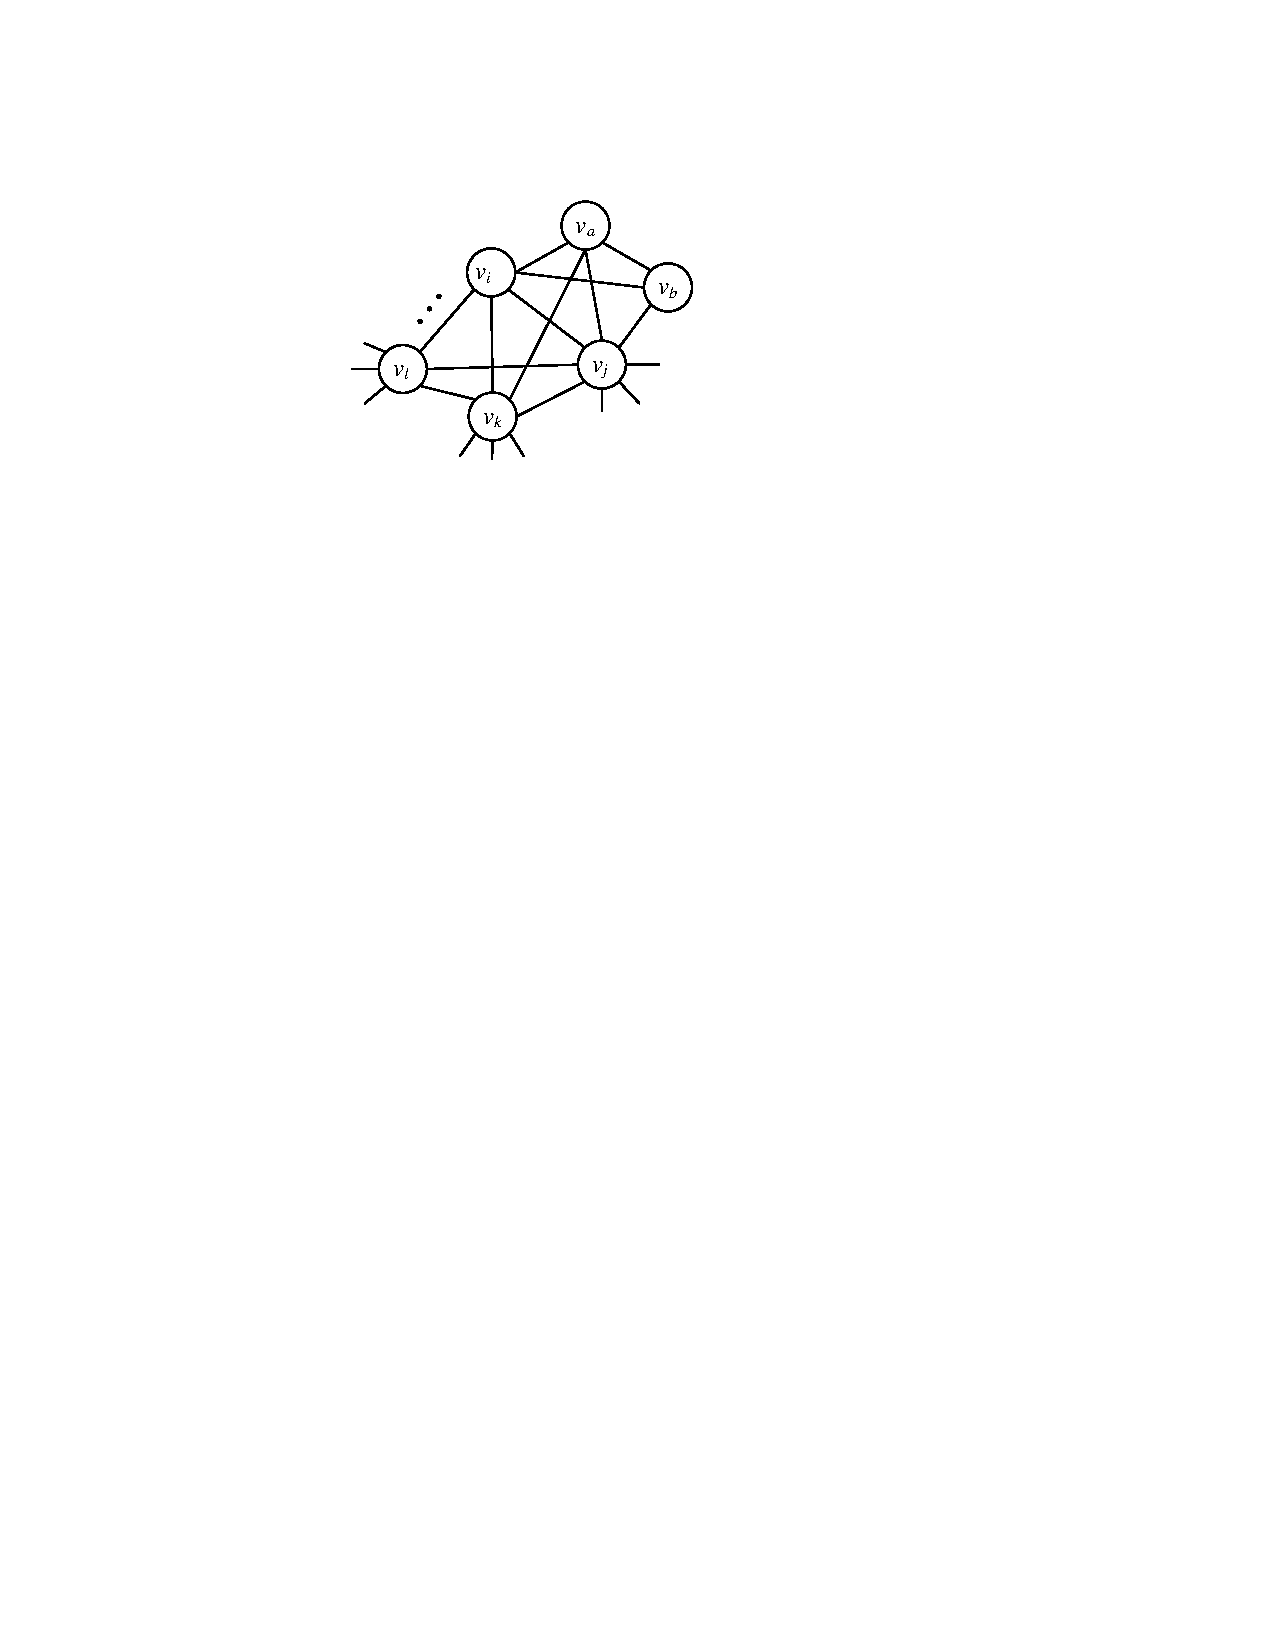
\includegraphics[width=2.4 in, height=1.5 in]{Ch3f2.pdf}
 \caption{ A fragment of a 3-tree}
 \label{fig:f3t1}
\end{figure}

 The following are basic properties of $k$-trees (for other properties, see e.g., \cite{golumbic2004algorithmic} and \cite{proskurowski1984separating})

\begin{lemma}\label{lem:1} \mbox{ }
\normalfont
\begin{enumerate}[noitemsep]
\item Every $k$-tree that is not a complete graph has at least two non-adjacent $k$-leaves.
\item Given a $k$-tree $G$ and a $k$-clique subgraph $H$ of $G$, there exists a $k$-leaf elimination sequence that reduces $G$ to $H$.
\item Given two non-adjacent nodes $u$ and $v$ of a $k$-tree $G$, a subgraph induced on any minimal $(u,v)$-separator is a $k$-clique. $\blacksquare$
\end{enumerate}
\end{lemma}

{\bf Partial $k$-Trees.} A partial $k$-tree is a $k$-tree possibly missing some edges. The classes of partial $k$-trees, for $k=1,2,3,\ldots$, form a hierarchy of graphs since any partial $k$-tree is also a partial $k+1$-tree. A \textit{leaf} of a partial $k$-tree $G$ is a node $x$ that is a $k$-leaf in some embedding of $G$ in a $k$-tree $\tilde{G}$ (thus, $deg_G(x)\leq k$). A \textit{perfect elimination} of a node $x$ from $G$ is the elimination of $x$ and its incident edges and the addition of the necessary edges to complete $N_G(x)$ to a clique. A \textit{$k$-perfect elimination sequence} $(k\mbox{-}PES)$ of a graph $G$ is an ordering $(v_1,v_2,\ldots,v_r)$ of $V(G)$ such that

\begin{enumerate}[noitemsep]
\item $deg_G(v_1)\leq k$, and
\item for $i=2,3,\ldots,$ the degree of $v_i$ is obtained by removing the sequence $v_1,\ldots,v_{i-1}$ is at most $k$.
\end{enumerate}

\begin{example}
\normalfont 
For the graph $G$ in figure \ref{fig:f3t2}, $(v_a,v_b,v_i,v_j,v_k,v_l)$ is a 3-$PES$. $\blacksquare$
\end{example}
\begin{figure}[!htb]
\centering
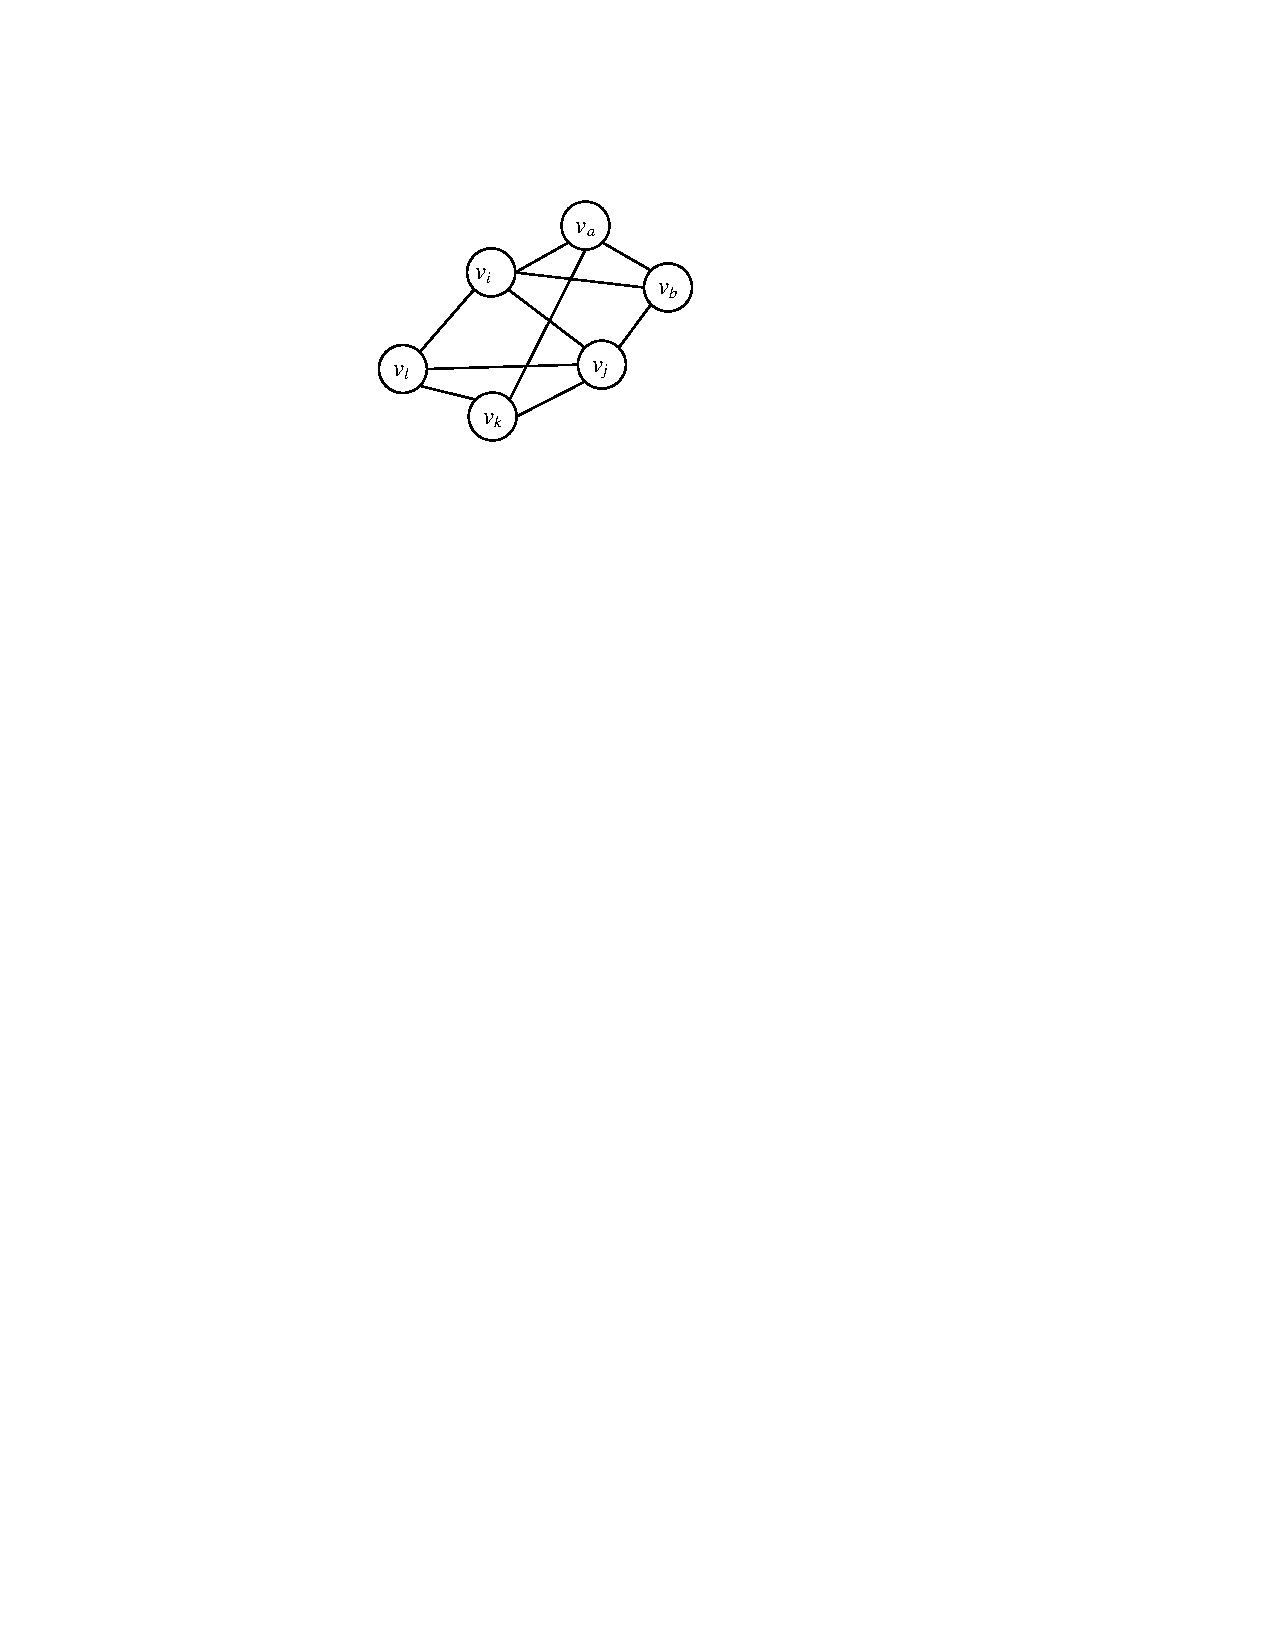
\includegraphics[width=2.4 in, height=1.5 in]{Ch2f2.pdf}
 \caption{ A partial 3-tree}
 \label{fig:f3t2}

\end{figure}
Every partial $k$-tree $G$ has a $k\mbox{-}PES$. Similar to Lemma \ref{lem:1} (1), every partial $k$-tree that is not a complete graph has at least two non-adjacent leaves. In Chapters 4 and 5, $G$ is a partial $k$-tree, for some $k$, of some sensor network that contains a sink node $s$. In any completion of $G$ to a $k$-tree $\tilde{G}$, the sink node appears in some $k$-clique $H$. By lemma \ref{lem:1}, one can find a $k$-$PES$ such that the sink node is the last node in the sequence. We henceforth deal with such $k$-$PES$.\\

{\bf Graphs with Bounded Tree-width.}
The work in \cite{robertson1986graph} has introduced the concept of graphs with bounded \textit{tree-width} in the context of resolving a particular graph theoretic conjecture. The concept is defined as follows.
\begin{definition}\normalfont \cite{robertson1986graph}
A \textit{tree-decomposition} of a graph $G$ is a family ($X_i:i\in I$) of subsets of $V(G)$, together with a tree $T$ with $V(T)=I$, with the following properties.
\begin{enumerate}[noitemsep]
\item $\displaystyle \bigcup_{i\in I} X_i =V(G)$.
\item Every edge of $G$ has both its ends in some $X_i$.
\item For $i,j,k \in I$, if $j$ lies on the path of $T$ from $i$ to $k$ then $X_i\cap X_k \subseteq X_j$. $\blacksquare$
\end{enumerate} 
\end{definition}

\begin{definition}
\normalfont
The \textit{width} of a tree-decomposition is $max(|X_i|-1:i\in I)$. $\blacksquare$
\end{definition}
\begin{definition}
\normalfont
The \textit{tree-width} of $G$ is the minimum $w \geq 0$ such that $G$ has a tree-decomposition of width $\leq w$. $\blacksquare$
\end{definition}

\begin{example}
\normalfont
Figure \ref{fig:GandT}(a) illustrates a graph $G$ having a tree-decomposition shown in figure \ref{fig:GandT}(b). The width of the tree decomposition is 3. One may verify that 3 is actually the tree-width of $G$. $\blacksquare$
\end{example}
\begin{figure}[!htb]
\centering
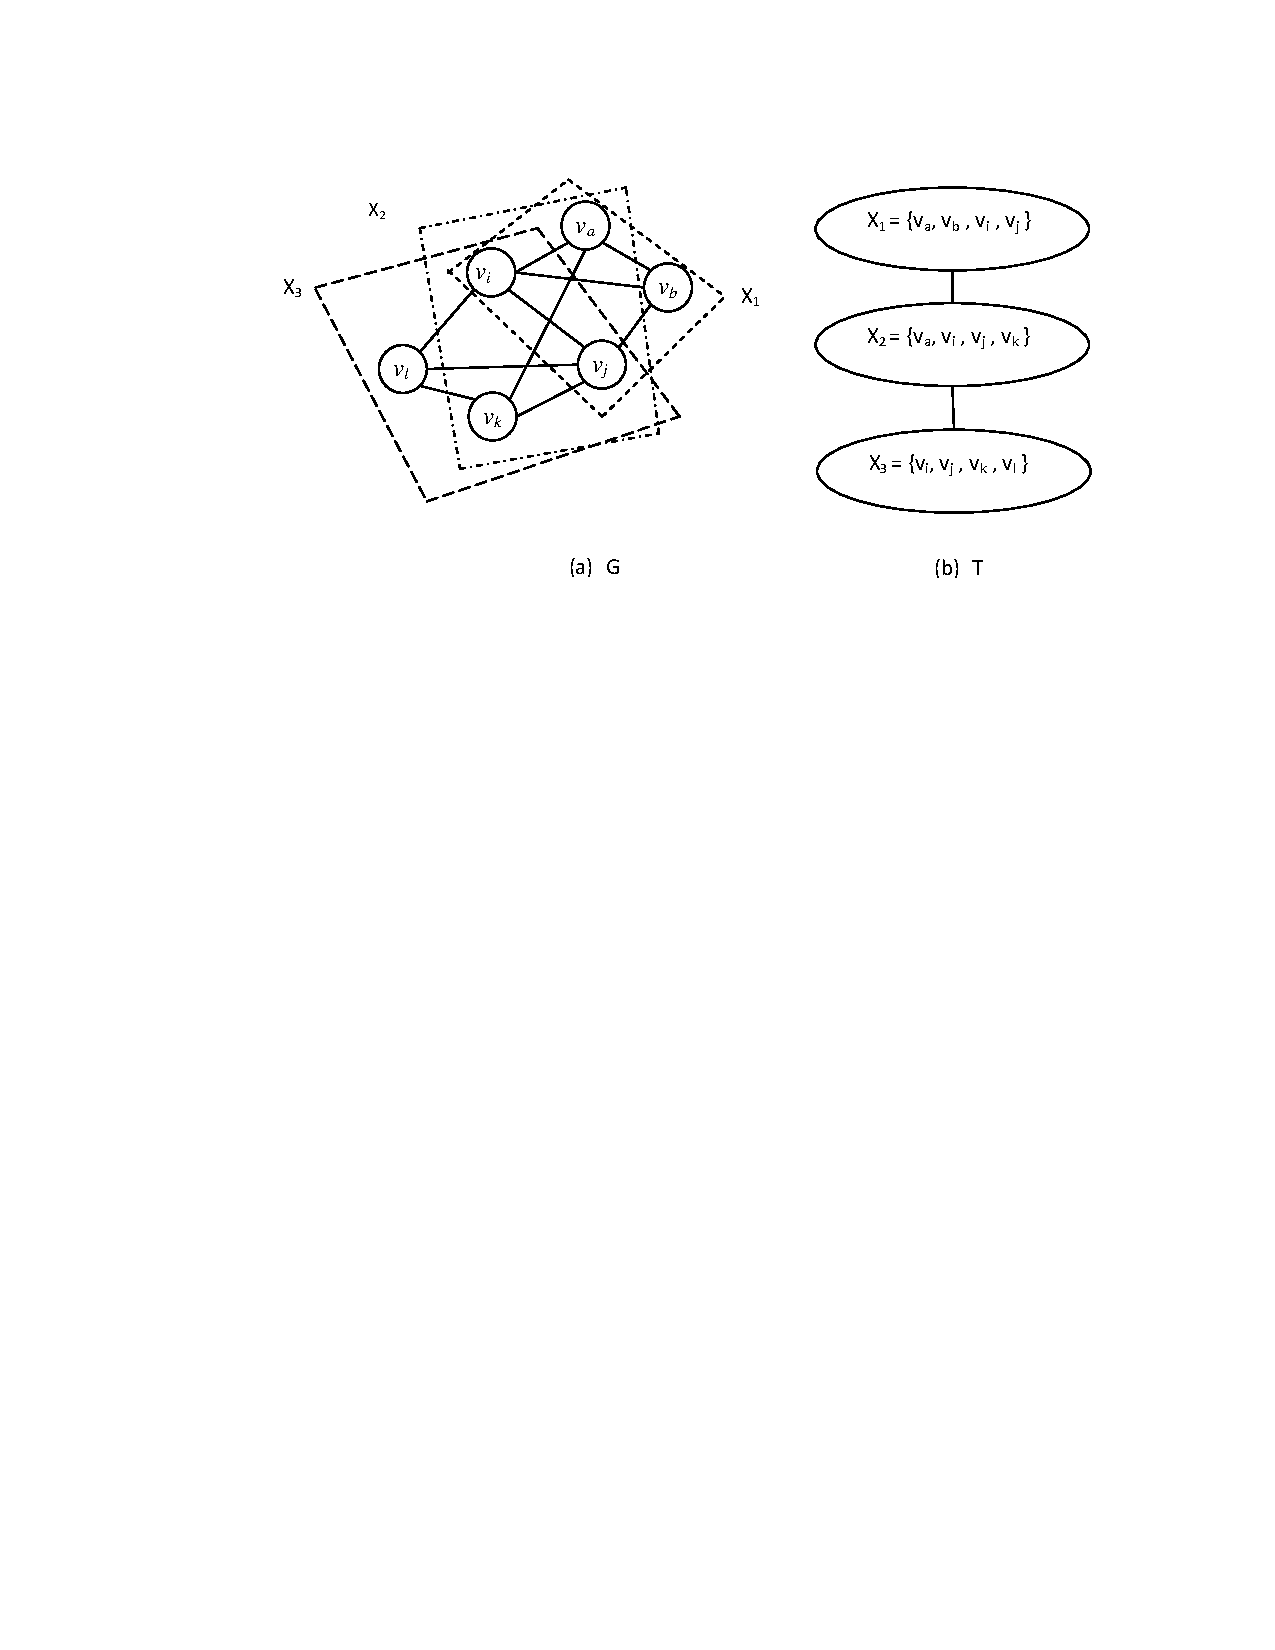
\includegraphics[width=5 in, height=2.2 in]{Ch2f3.pdf}
 \caption{ Tree decomposition}
 \label{fig:GandT}

\end{figure}
The following result is mentioned in \cite{brandstadt1999graph}.
\begin{theorem}
\normalfont
$G$ has tree-width $\leq k$, if and only if $G$ is a partial $k$-tree. $\blacksquare$ 
\end{theorem}

{\bf Relation to Other Graph Classes:}  Several classes of graphs surveyed in \cite{brandstadt1999graph} are known to be partial $k$-trees for fixed $k$. For example, 
\begin{itemize}[noitemsep]
\item  Cactus graphs, series-parallel graphs, and outerplanar graphs are partial 2-trees.
\item Halin graphs and Y-$\Delta$ graphs are partial 3-trees.
\item A chordal graph $G$ with maximum clique of $\omega (G)$  nodes is a  partial $(\omega (G)-1)$-tree. A graph is chordal if it has no induced cycle on 4 or more nodes.
\item An $n\times n$ grid (on $n^2$ nodes), $n\geq 2$, has tree-width $n$.
\end{itemize}
\section{Dynamic Programming on Partial $k$-Trees}
\label{ch2:dpk}
The theory of partial $k$-trees and graphs with bounded tree-width is rich with dynamic programming algorithms for solving many problems that are NP-complete in general.
The work of \cite{arnborg1989linear} is an example survey paper of such algorithm published in or before 1989.
%
More recently, there has been work on obtaining unifying results that show classes of problems that admit polynomial time solutions on partial $k$-trees, for fixed $k$.
%
Example of such unifying results include the work of \cite{bodlander1988} and \cite{arnborg1991easy}.

The approach used in such results relies on formalizing graph and network properties as logical statements in a particular logic system. 
Such approaches are not intended to provide optimized algorithms for solving any particular problem at hand, or implementing a direct solution. It is often more fruitful to construct a direct algorithm for handling a given problem of interest.
In the rest of the section, we review a dynamic programming algorithm result due to \cite{wald1983steiner} for solving the Steiner tree problem on partial 2-trees.
This dynamic programming algorithm has inspired the design of many subsequent algorithms for solving other NP-complete problems on partial $k$-trees. 
A Steiner tree can be defined as follows.
\begin{definition}
\normalfont
Given a graph $G = (V,E)$ with positive integer edge costs, and a set of target nodes $V_{target}\subseteq V$, a Steiner tree, denoted $ST(G,V_{target} )$, is a subtree $G' = (V',E')$ satisfying
\begin{enumerate}[noitemsep]
\item  $V_{target} \subseteq V'\subseteq V$ ,
\item the sum of edge costs in $E'$ is minimum over all subtrees satisfying (1). $\blacksquare$
\end{enumerate}
\end{definition}

The algorithm devised in \cite{wald1983steiner} works as follows. The graph is reduced by repeated deletion of degree-2 vertices until the graph which remains is a single edge. During this vertex elimination procedure, the algorithm summarize information about the triangle
$\{ x , y , z \}$ , where $y$ has degree 2, on the arcs $(x,z)$ and $( z , x )$ , prior to deleting $y$. This
summary information encodes information about Steiner trees in the subgraph of the 2-tree which has thus far been reduced onto the edge $\{x, z \}$. With each edge $\alpha = (x, y)$ of $G$, the algorithm associates six cost measures, which summarize the cost incurred so far of the subgraph $S$ which has been reduced onto the edge $(x , y )$ \cite{wald1983steiner}:
\begin{enumerate}[noitemsep]
\item $st(\alpha)$ is the minimum cost of a Steiner tree for $S$, in which $x$ and $y$ appear in the same tree.
\item $dt(\alpha)$ is the minimum cost of two disjoint trees for $S$ including all targets, one tree involving $x$ and the other $y$.
\item  $yn(\alpha)$ is the minimum cost of a Steiner tree for $S$, which includes $x$ but not $y$.
\item $ny(\alpha)$ is the minimum cost of a Steiner tree for $S$, which includes $y$ but not $x$.
\item $nn(\alpha)$ is the minimum cost of a Steiner tree for $S$, which includes neither $x$ nor $y$.
\item $none(\alpha)$ is the cost of omitting all vertices of $S$ from a Steiner tree.
\end{enumerate}
The six measures are initialized as follows:
\begin{enumerate}[noitemsep] 
\item $st(\alpha)=cost(\alpha)$
\item $dt(\alpha)=0$
\item  $yn(\alpha)=BIG$ if $y\in V_{target},0$ otherwise.
\item $ny(\alpha)=BIG$ if $x\in V_{target},0$ otherwise.
\item $nn(\alpha)=BIG$ if $x\in V_{target}$ or $y\in V_{target},0$ otherwise.
\item $none(\alpha)$ if $x\in V_{target}$ or $y\in V_{target},0$ otherwise.
\end{enumerate}
A cost of $BIG$ is incurred whenever an attempt is made to omit a target vertex.
The initial edge costs are used to update edge costs as the graph is reduced. The graph is reduced by repeated deletion of degree-2 vertices. So, suppose at some point there is a triangle $\{ x , y , z \}$ in which $y$ is a degree-2 vertex, and valid costs have been computed for $( x , y )$ and $(y,z)$. The algorithm uses these values to update the costs for $( x , z )$ prior to deleting $y$, as follows. Let $L = (x,y)$, $R = (y , z )$, and $M = ( x , z )$. The costs are updated for $M$ using the following recurrences \cite{wald1983steiner}:

\begin{enumerate}[noitemsep]
\item $st(M)=min[st(M)+min[dt(L)+st(R),st(L)+dt(R),yn(L)+ny(R)],dt(M)+st(L)+st(R)]$,
\item $dt(M)=dt(M)+min[dt(L)+st(R),st(L)+dt(R),yn(L)+ny(R)]$,
\item $ny(M)=ny(M)+min[ny(L)+st(R),none(L)+ny(R)]$,
\item $yn(M)=yn(M)+min[yn(L)+none(R),st(L)+yn(R)]$,
\item $nn(M)=min[nn(M)+none(L)+none(R),none(M)+nn(L)+none(R),none(M)+none(L)+nn(R),none(M)+ny(L)+yn(R)]$,
\item $none(M)=none(M)+none(L)+none(R)$,
\end{enumerate}



An alternative approach to present the above algorithm is to store the six measures associated with edge $\alpha=(x,y)$ in a table, denoted $T_{x,y}$. The table provides key-value mappings. Roughly speaking, the keys replace the use of some of the names $st,dt,yn, $ etc. with set notation. Not all names correspond to keys in this formulation. Examples of names that correspond to keys are:

$st=\{x,y\}_1,dt=\{x\}_1\{y\}_1, yn=\{x\}_1\{y\}_0, \mbox{ and } ny=\{x\}_0\{y\}_1$.


As can be seen, each key contains a partition of the set $\{x,y\}$. To explain the keys, let $S$ be a subgraph reduced onto the edge $\alpha=(x,y)$ in some iteration of the algorithm, and let $S'\subseteq S$ be a subgraph of $S$ that is a candidate for appearing in a final solution. We now have:

\begin{itemize}[noitemsep]
\item The key $\{x,y\}_1$ is associated with a minimum cost $S'$ such that both $x$ and $y$ appear in one connected component of $S'$, and this component has at least one target node (counting $x$ and $y$ as possible target nodes). 
\item The key $\{x\}_1\{y\}_0$ is associated with a minimum cost $S'$ such that  $x$ and $y$ appear in two different components of $S'$, and only the component that includes $x$ contains one, or more, target nodes.
\end{itemize}
In this alternative approach, the above recurrences are replaced by functions that merge 3 tables $T_{x,y}, T_{y,z}$ and $T_{x,z}$ into an updated $T_{x,z}$ table.

\section{Set Partitions}
\label{sec:setPartitions}
The dynamic programs devised in the rest of the thesis make heavy use of set partitioning, as explained below. Given a set $X$, a partition of $X$ is a set $\{X_1,X_2,\ldots, X_r\}$, $1\leq r\leq |X|$ such that 
\begin{enumerate}
\item $X=\displaystyle \bigcup_{i=1,2,\ldots,r} X_i$.
\item The $X_i$s are pairwise disjoint.
\end{enumerate}
In our algorithm, $X$ is a set of nodes in a $k$-clique, and the partition of $X$ are used as part of states of dynamic programs.
%
The number of all possible partition of a set $X$ on $n$ elements are known as Bell numbers, denoted $B_n$ (see for example \cite{brualdi2009introduction}).
The first few Bell numbers are 
\begin{center}
$\begin{array}[t]{l}
B_0=B_1=1,B_2=2,\\
B_3=5,B_4=15,B_5=52,\\
B_6=203,B_7=877,B_8=4140, \ldots \\
\end{array}$
\end{center}
Bell numbers satisfy the following recurrence equation:
\begin{center}

$ B_0=1, B_1=1 \mbox{ and } B_{n+1}=\displaystyle \sum_{k=0}^n (\begin{array}{l} n \\ k \end{array})B_k.
$
\end{center}

\section{Finding Good Partial $k$-Tree Subgraphs}
\label{sec:fgpkts}

The algorithms presented in Chapters 3 to 5 can be used to derive lower bounds on the $Conn(G)$ and $Conn(G,n_{req})$ measures. This is done by
\begin{enumerate}
\item  constructing a graph $G$ that underlies the structure of a given probabilistic graph of the problem instance at hand (as explained in subsequent chapters), and
\item  identifying a subgraph $G'$ of $G$ that is a partial $k$-tree, of some user specified $k$.
\end{enumerate}
Under simple assumptions, we have $Conn(G')\leq Conn(G)$ (or, $Conn(G',n_{req})\leq Conn(G,n_{req})$).
So $Conn(G')$, or $Conn(G',n_{req})$, is a lower bound on the required solution.

Ideally, one would prefer to use a subgrpah $G'$ that gives the best possible lower bound. The problem of finding such subgraph is a complex graph problem. This class of problems is related to the following classes of problems.

\begin{enumerate}[noitemsep]
\item {\bf Recognizing  Partial $k$-Trees:} Given a graph $G$, and an integer $k\geq 1$, is $G$ a partial $k$-tree?\\
\begin{itemize}
\item The work of \cite{arnborg1987complexity} shows $O(n^{k+2})$ algorithm for solving the problem. If $k$ is not fixed, then \cite{arnborg1987complexity} shows that the problem is NP-complete.

\item For any fixed  $k$, the work of \cite{bodlaender1993linear} improves on the above result by showing a linear time recognition algorithm.
\end{itemize}
The above results produce also a $k$-$PES$ if one exists.\\

\item {\bf Edge Deletion Problem (EDP) to Obtain a Partial $k$-Tree:}  Given a graph $G$, and an integer $k$, find the minimum number of edges whose deletion gives a partial $k$-tree.
\begin{itemize}
\item For $k=1$, the problem is simple.
\item For $k\geq 2$, the problem is NP-complete (see, e.g. the work of \cite{el1988complexity} and the references therein)
\end{itemize}
\end{enumerate}

In the absence of known algorithms to find the required best subgraphs, we resort to using heuristic algorithms. In Chapters 3 to 5, we experiment with partial $k$-tree subgraphs ($k=1,2, \mbox{ and }3$) obtained using the following methods. We assume that $G$ is a connected graph.


\nwline
{\bf The Random Method.} Subgraphs obtained using the random method are used as baseline cases for comparisons. This method constructs a partial $k$-tree subgraph for $k=1,2, \mbox{ and }3,$ as follows.
\begin{itemize}
\item {\bf Case $k=1$.} Choose any spanning tree.
\item {\bf Case $k=2$.} Choose a spanning tree $G'\subseteq G$. Fix an ordering of the remaining edges not in $G'$. For each edge $e$ in the fixed order, test whether $G'+e$ is a partial 2-tree. If yes, add $e$ to $G'$, and proceed to the next edge in the fixed order.
\item {\bf Case $k=3$.} Build a partial 2-tree $G'\subseteq G$ as in case $k=2$, and let $S=(v_1,v_2, \ldots,v_{n-2})$ be a $2$-$PES$ of $G'$. Fix an ordering of the edges not in $G'$. For each edge $e$ in the fixed order, test whether $G'+e$ is a partial 3-tree with $S$ being a 3-$PES$.  If yes, add $e$ to $G'$, and proceed to the next edge in the fixed order.
\end{itemize}
\nwline
{\bf The Greedy Method.} Here, we associate with each link $(x,y)\in E_G$ a probability, denoted $p(x,y)$, of having the link $(x,y)$ present, given the locality sets $Loc(x)$ and $Loc(y)$. For convenience of using a minimum spanning tree algorithm, we transform each non-zero edge probability $p(x,y)> 0$ into edge cost using the relation $cost(x,y)=-\log p(x,y)$. The greedy method constructs partial $k$-tree subgraphs for $k=1,2,$ and $3$ as follows.
\begin{itemize}
\item {\bf Case $k=1$:} Choose a minimum spanning tree using the above edge costs.
\item {\bf Case $k=2$ and $3$:} As in cases $k=2$ and $3$, respectively, of the random method, where we sort the remaining edges in a non-decreasing order of their costs to obtain the fixed order
\end{itemize}



\section{Concluding Remarks}
\label{ch2:sum}
In this chapter we have presented some background information on $k$-trees and partial $k$-trees that serves as an introduction to the algorithms developed in subsequent chapters.